% =====================================================================
% StaticKD -- SOURCE of the paper (modular, with \val{key} numbers). Do not submit this file.
% python scripts/build_paper.py  ->  jurnal_final/main.tex (one file, literal numbers) + jurnal_final/figures/
% Numbers: generated by notebooks/StaticKD_IPTC_final.ipynb into results/final/paper_generated/.
% Content: research_final/paper_quality_check_filled.md (Values); style: research_final/ai_text_criteria_to_be_avoided.txt
% =====================================================================
\documentclass[journal]{IEEEtran}

\usepackage[T1]{fontenc}
\usepackage[utf8]{inputenc}
\usepackage[nocompress]{cite}
\usepackage{amsmath,amssymb}
\usepackage{graphicx}
\usepackage{booktabs}
\usepackage{multirow}
\usepackage{array}
\usepackage{xcolor}
\usepackage[hyphens]{url}
\usepackage{tikz}
\usetikzlibrary{positioning,arrows.meta,fit,calc}

\DeclareRobustCommand{\todo}[1]{{\color{red}[TODO: #1]}}
\newcommand{\eng}[1]{#1}
\makeatletter
\newcommand{\rows}[1]{\@@input #1 }
\makeatother
\input{generated/numbers}
% Table environments whose bodies are generated by the notebook (generated/tab_*.tex).

\newcommand{\TabMain}{%
\begin{table*}[!t]
\caption{Main Results. Macro-F1 [95\% CI] and Accuracy on the Development Set (EMMediaTopic Dev, GPT-4o Labels), Agreement with the Teacher on CC-News Held-Out, and Results on the Unified Test Set (\val{ts.langs} Languages, Independent Labels). Test CIs from the Site-Cluster Bootstrap}
\label{tab:main}
\centering
\footnotesize
\setlength{\tabcolsep}{3.5pt}
\begin{tabular}{@{}lccccccc@{}}
\toprule
 & \multicolumn{2}{c}{dev (4 languages)} & held-out & \multicolumn{4}{c}{unified test (\val{ts.langs} languages)} \\
\cmidrule(lr){2-3}\cmidrule(lr){4-4}\cmidrule(lr){5-8}
Model & Macro-F1 [95\% CI] & Accuracy & Agreement & Macro-F1 [95\% CI] & Accuracy & Macro-F1/language & \% teacher \\
\midrule
\rows{generated/tab_main}
\bottomrule
\end{tabular}
\end{table*}}

\newcommand{\TabSig}{%
\begin{table*}[!t]
\caption{Paired Tests of StaticKD Against Other Models ($\Delta$ = StaticKD $-$ Comparison Model; $p$ Holm-Corrected Within Each Set; $b/c$ = Documents Correct Only for StaticKD / Only for the Comparison Model)}
\label{tab:sig}
\centering
\footnotesize
\begin{tabular}{@{}llccccc@{}}
\toprule
Set & StaticKD vs & $\Delta$macro-F1 [95\% CI] & $p$ bootstrap & $\Delta$accuracy & McNemar $b/c$ & $p$ McNemar \\
\midrule
\rows{generated/tab_sig}
\bottomrule
\end{tabular}
\end{table*}}

\newcommand{\TabGroups}{%
\begin{table*}[!t]
\caption{Test Macro-F1 by Subgroup. Last Column: StaticKD Macro-F1 as a Percentage of the Teacher Macro-F1 in the Same Subgroup}
\label{tab:groups}
\centering
\footnotesize
\setlength{\tabcolsep}{3.5pt}
\input{generated/tab_groups}
\end{table*}}

\newcommand{\TabSources}{%
\begin{table*}[!t]
\caption{Test Macro-F1 by Source of the Unified Test Set. MN-DS Is the Only Source Annotated Directly With IPTC Topics; MasakhaNEWS Is Human-Annotated Under Its Own Scheme. Last Column: StaticKD as a Percentage of the Teacher}
\label{tab:sources}
\centering
\footnotesize
\setlength{\tabcolsep}{3.5pt}
\resizebox{\textwidth}{!}{\input{generated/tab_sources}}
\end{table*}}

\newcommand{\TabAblation}{%
\begin{table*}[!t]
\caption{Ablations, Temperature, and Exploratory Variants (One Student, No Ensemble). Mean $\pm$ Standard Deviation Over Seeds; $^{*}$: Different From the Final Recipe (Welch, Holm, $p<0.05$)}
\label{tab:ablation}
\centering
\footnotesize
\begin{tabular}{@{}lccccc@{}}
\toprule
Variant & Seeds & Dev macro-F1 & Held-out agreement & Test macro-F1 & Test accuracy \\
\midrule
\rows{generated/tab_ablation}
\bottomrule
\end{tabular}
\end{table*}}

\newcommand{\TabAblationGroups}{%
\begin{table}[!t]
\caption{Macro-F1 of Selected Variants by the Amount of Distillation Data in the Language of the Article (Test Set; Mean Over Seeds)}
\label{tab:ablation-groups}
\centering
\footnotesize
\setlength{\tabcolsep}{3pt}
\resizebox{\columnwidth}{!}{%
\begin{tabular}{@{}lcccc@{}}
\toprule
Variant & Dev & Sufficient ($\ge$500) & Few ($<$500) & None (0) \\
\midrule
\rows{generated/tab_ablation_groups}
\bottomrule
\end{tabular}}
\end{table}}

\newcommand{\TabEff}{%
\begin{table*}[!t]
\caption{CPU Efficiency (Pinned P-Cores; Sample From the Unified Test Set; 1c/4c = 1/4 Cores)}
\label{tab:eff}
\centering
\footnotesize
\resizebox{\textwidth}{!}{%
\begin{tabular}{@{}lcccccl@{}}
\toprule
Model & Latency p50 / p95, 1c (ms) & Throughput 1c (doc/s) & Throughput 4c (doc/s) & Model RAM (MB) & File (MB) & Dependencies \\
\midrule
\rows{generated/tab_eff}
\bottomrule
\end{tabular}}
\end{table*}}

\newcommand{\TabFactors}{%
\begin{table}[!t]
\caption{Factors Behind Per-Language Performance}
\label{tab:factors}
\centering
\footnotesize
\setlength{\tabcolsep}{3pt}
\resizebox{\columnwidth}{!}{%
\begin{tabular}{@{}lcc@{}}
\toprule
Test & Statistic & $p$ \\
\midrule
\rows{generated/tab_factors}
\bottomrule
\end{tabular}}
\end{table}}

\newcommand{\TabCascade}{%
\begin{table}[!t]
\caption{Cascade StaticKD $\rightarrow$ ONNX Int8 Teacher on the Test Set (Effective Single-Core Throughput)}
\label{tab:cascade}
\centering
\footnotesize
\setlength{\tabcolsep}{2.5pt}
\resizebox{\columnwidth}{!}{%
\begin{tabular}{@{}lccccc@{}}
\toprule
$\theta$ & StaticKD share & Accuracy on share & Macro-F1 & Accuracy & doc/s \\
\midrule
\rows{generated/tab_cascade}
\bottomrule
\end{tabular}}
\end{table}}

% Tables written by hand (TabRelated, TabLicense) or whose rows come from generated/ (TabTestset, TabHparams).

\newcommand{\TabRelated}{%
\begin{table*}[!t]
\caption{Position of StaticKD Relative to Related Approaches}
\label{tab:related}
\centering
\footnotesize
\setlength{\tabcolsep}{4pt}
\resizebox{\textwidth}{!}{%
\begin{tabular}{@{}llccccc@{}}
\toprule
Approach & Model at inference time & Multilingual & Cross-lingual transfer & No deep learning library & CPU cost reported & IPTC labels \\
\midrule
Kuzman \& Ljube\v{s}i\'c~\cite{kuzman2025llm} & XLM-R-large (\val{teacher.params}M parameters) & yes & yes & no & no & yes \\
LoRA/PEFT~\cite{hu2022lora,razuvayevskaya2024peft} & full transformer backbone & partly & yes & no & no & no \\
DistilBERT, MiniLMv2~\cite{sanh2019distilbert,wang2021minilmv2} & 6-layer transformer & partly & yes & no & partly & no \\
Sparse Distillation~\cite{ye2022sparse} & deep averaging network + n-gram table & no (en) & no & yes & yes & no \\
Model2Vec~\cite{tulkens2024model2vec}, Wada et al.~\cite{wada2025static} & static embeddings, optional MLP classifier & yes & yes & yes & partly & no \\
fastText~\cite{joulin2017bag} & bag of n-grams & per language & no & yes & yes & no \\
StaticKD (proposed) & table of 17 logits per token & yes & yes & yes & yes & yes \\
\bottomrule
\end{tabular}}
\end{table*}}

\newcommand{\TabTestset}{%
\begin{table}[!t]
\caption{Composition of the Unified Test Set by Source}
\label{tab:testset}
\centering
\footnotesize
\setlength{\tabcolsep}{3pt}
\resizebox{\columnwidth}{!}{%
\begin{tabular}{@{}llrrr@{}}
\toprule
Source & Label origin & Articles & Languages & Sites/sources \\
\midrule
\rows{generated/tab_testset}
\bottomrule
\end{tabular}}
\end{table}}

\newcommand{\TabHparams}{%
\begin{table}[!t]
\caption{Hyperparameters of All Models}
\label{tab:hparams}
\centering
\footnotesize
\setlength{\tabcolsep}{3pt}
\resizebox{\columnwidth}{!}{%
\begin{tabular}{@{}ll@{}}
\toprule
Component & Value \\
\midrule
\rows{generated/tab_hparams}
\bottomrule
\end{tabular}}
\end{table}}

\newcommand{\TabLicense}{%
\begin{table}[!t]
\caption{Licenses of the Assets Used and Released}
\label{tab:license}
\centering
\footnotesize
\setlength{\tabcolsep}{3pt}
\resizebox{\columnwidth}{!}{%
\begin{tabular}{@{}ll@{}}
\toprule
Asset & License \\
\midrule
Teacher \texttt{classla/multilingual-IPTC-news-topic-classifier} & CC BY-SA 4.0 \\
Embeddings \texttt{minishlab/potion-multilingual-128M} & MIT \\
MasakhaNEWS & CC BY-NC 4.0 \\
MN-DS, L3Cube-IndicNews, IndoNews, Amharic news & CC BY 4.0 \\
Bangla news~\cite{hossain2025banglanews} & not stated on the dataset card \\
EMMediaTopic 1.0 & CC BY-SA 4.0 \\
CC-News 2019--2021, CC-NEWS 2024--2026 & Common Crawl terms of use \\
\midrule
StaticKD code (release) & MIT \\
StaticKD models (release) & CC BY-SA 4.0 (inherited from the teacher) \\
Test-set manifest (release) & CC BY-SA 4.0 \\
\bottomrule
\end{tabular}}
\end{table}}


\emergencystretch=1.5em

\begin{document}

\title{StaticKD: Distilling a Multilingual IPTC News Topic Classifier into a Static Token-Logit Table for Lightweight CPU Inference}

\author{Obi~Kastanya and Ananta~Dwi~Prayoga~Alwy%
\thanks{O. Kastanya and A. D. P. Alwy are with the Department of Informatics Engineering, Sepuluh Nopember Institute of Technology, Surabaya, Indonesia (e-mail: 6025252015@student.its.ac.id; 6025252007@student.its.ac.id). Corresponding author: O. Kastanya. This work received no specific funding.}}

\markboth{IEEE Access (draft)}%
{Kastanya and Alwy: StaticKD, Multilingual IPTC News Topic Classification on CPU}

\maketitle

\begin{abstract}
Filtering news by the International Press Telecommunications Council (IPTC) Media Topic taxonomy needs a classifier that is cheap to run on a multilingual stream of articles. The open multilingual IPTC classifier, based on XLM-RoBERTa-large, takes \val{eff.teacher_onnx_int8.latency_ms_p50_1c} to \val{eff.teacher.latency_ms_p50_1c} milliseconds per article on one processor core. It is distilled into StaticKD, a student built on multilingual static embeddings whose linear head is folded into the embedding table, so the whole model is one table of 17 logits per token. The teacher labels \val{data.pool.docs} unlabeled articles in \val{data.pool.langs} languages. A test set of \val{ts.docs} articles in \val{ts.langs} languages, labeled by human annotators or by the sections that newsroom editors assigned and mapped onto the IPTC tree, allows evaluation without labels from any model. On this test set StaticKD reaches a macro-F1 of \val{statickd.test.macro}, or \val{statickd.test.pct_teacher} of the teacher score of \val{teacher.test.macro}. It classifies \val{eff.statickd.docs_per_sec_1c} articles per second per core, about \val{eff.statickd.speedup_onnx} times faster than the 8-bit quantized teacher, with a \val{final.size}-megabyte model, and it is more accurate than fastText and a linear support vector machine distilled on the same data. Ablations with five seeds per variant show that accuracy comes from multilingual distillation data and cross-lingually aligned embeddings, while hard labels match soft labels. Transfer to languages absent from the distillation data is carried by embedding rows that training never updates, and fine-tuning the embeddings trades this transfer for in-distribution fit. StaticKD is weakest on languages missing from both the distillation data and the pre-training data of the teacher.

\end{abstract}

\begin{IEEEkeywords}
Efficient inference, knowledge distillation, multilingual text classification, news topic classification, static embeddings.
\end{IEEEkeywords}

\section{Introduction}
\label{sec:introduction}
\IEEEPARstart{N}{ews} analytics pipelines assign articles to standard topics early, so that the more expensive stages only process the topics that matter. The taxonomy most used by news agencies is Media Topic of the International Press Telecommunications Council (IPTC). Its top level has 17 topics, such as \emph{politics}, \emph{economy, business and finance}, and \emph{sport}~\cite{iptc2024mediatopics,kuzman2025llm}.

Kuzman and Ljube\v{s}i\'c~\cite{kuzman2025llm} released the first open multilingual IPTC classifier. They labeled articles in four languages with GPT-4o and used these labels to fine-tune XLM-RoBERTa-large~\cite{conneau2020xlmr}. The resulting model matches GPT-4o on a human-annotated test set. A follow-up study by the same group concluded that fine-tuned encoders are more practical than large language models (LLMs) for large-scale annotation~\cite{kuzman2025southslavic}. An encoder with \val{teacher.params}~million parameters is still expensive without a graphics processing unit (GPU). On one central processing unit (CPU) core the model needs \val{eff.teacher.latency_ms_p50_1c}~ms per article, and its fastest CPU configuration, an Open Neural Network Exchange (ONNX) export quantized to 8-bit integers (int8), still needs \val{eff.teacher_onnx_int8.latency_ms_p50_1c}~ms (Section~\ref{sec:res-eff}). Neither study reports this inference cost, although inference accounts for a large share of the computing demand and energy use of machine learning in production, for example 60\% of the machine learning energy use reported by Google~\cite{luccioni2024power}.

The target is a topic classifier that covers many languages, runs in milliseconds per article on an ordinary CPU, and has a small footprint and few dependencies. Existing options fall short of this. Small distilled transformers~\cite{sanh2019distilbert,wang2021minilmv2} gain about one order of magnitude. In the CPU benchmark of this study, MiniLM-L6 is \val{eff.minilm_kd.speedup_onnx} times faster than the ONNX int8 teacher. Int8 quantization alone gives a factor of \val{eff.teacher_onnx_int8.speedup_pt} over PyTorch fp32. fastText~\cite{joulin2017bag} is much faster, but it learns its embeddings from scratch and therefore does not transfer across languages. This matters here because labeled IPTC data exists for only four languages.

This paper proposes StaticKD, which distills~\cite{hinton2015distilling} the XLM-R-large IPTC classifier into a student that, after training, is a single table of 17 logits per token. A teacher that works across languages can label unlabeled news in any language at no annotation cost. Multilingual static embeddings distilled from sentence encoders~\cite{tulkens2024model2vec,wada2025static,chen2024bgem3} place translation equivalents close to each other, and looking them up costs almost nothing. News topics are also strongly lexical, which keeps bag-of-words representations competitive for topic classification~\cite{galke2022bow}. Because the classification head of StaticKD is linear, the averaged embedding and the head can be folded into a token table. Inference then reduces to tokenization and averaging table rows, which NumPy handles.

A multilingual claim requires a multilingual evaluation with labels that do not come from the teacher. The human test set of Kuzman and Ljube\v{s}i\'c is not public and covers four languages. SIB-200~\cite{adelani2024sib200} covers 205 languages, but its items are short sentences with a non-IPTC taxonomy. To fill this gap, a unified test set of \val{ts.docs} articles in \val{ts.langs} languages is built. It combines CC-NEWS articles from 2024 to 2026 that carry their newsroom section in schema.org metadata~\cite{guha2016schema} with public datasets labeled by humans or by publisher categories~\cite{adelani2023masakhanews,petukhova2023mnds,mirashi2023indicnews,hossain2025banglanews}. The labels are editorial decisions of publishers or annotators, translated onto the official IPTC tree. No model that reads the article text is involved.

This study addresses four research questions (RQs).
\begin{itemize}
  \item \textbf{RQ1 (cost):} What is the CPU inference cost of the IPTC teacher, and how much does StaticKD reduce it?
  \item \textbf{RQ2 (accuracy):} How much of the teacher accuracy does StaticKD retain on labels that do not come from the teacher, compared with baselines of similar cost, namely fastText and a support vector machine (SVM) on term frequency--inverse document frequency (TF-IDF) features, and with baselines of higher cost, namely MiniLM-L6 and DistilmBERT?
  \item \textbf{RQ3 (components):} Which distillation components determine the accuracy of this very-low-capacity student: soft labels, multilingual data, embedding initialization, embedding fine-tuning, token dropout, temperature, or ensembling?
  \item \textbf{RQ4 (generalization):} On which languages, labels, and label sources is StaticKD weak, and which factors explain it?
\end{itemize}

Distilling into a student of such low capacity also shows where its accuracy comes from. The knowledge that matters comes from the coverage of the transfer set and from the aligned initialization, not from the shape of the soft labels. Hard labels match soft labels, and a high temperature hurts. Transfer to languages that never appear in the distillation data is carried by embedding rows that training never updates, which works because they share a space with the trained rows. Fine-tuning the embeddings trades this transfer for in-distribution fit, a representation drift that a development set in the training languages cannot detect.

The contributions of this paper are as follows.
\begin{enumerate}
  \item A multilingual IPTC test set of \val{ts.docs} articles in \val{ts.langs} languages whose editorial labels do not come from the teacher. It comes with a section-to-IPTC mapping table that is validated automatically and reviewed by the first author, cross-source deduplication, a contamination check against all training data, and site-cluster bootstrap confidence intervals, and it can be reused to evaluate other IPTC classifiers.
  \item The findings above, supported by ablations with five seeds per variant and by analyses by language, label, label origin, and source, including languages that are absent from the distillation data.
  \item StaticKD, a recipe that distills a multilingual transformer teacher into a token-logit table initialized from cross-lingual static embeddings. The final model takes \val{final.size}~MB, needs only \texttt{numpy} and \texttt{tokenizers}, and processes \val{eff.statickd.docs_per_sec_1c} articles per second per core. An ensemble of seeds folds into the same table at no extra inference cost. Its accuracy--cost trade-off is compared with nine configurations from six model families, measured on CPU only with core pinning for a hybrid CPU.
  \item A release of the code, a notebook that reproduces every number in this paper, the models, and the test-set manifest.
\end{enumerate}

Section~\ref{sec:related} reviews related work, Section~\ref{sec:method} describes the data, test set, method, and evaluation protocol, Section~\ref{sec:results} presents the results, Section~\ref{sec:discussion} discusses them, Section~\ref{sec:limitations} lists the limitations, and Section~\ref{sec:conclusion} concludes.


\section{Related Work}
\label{sec:related}
\subsection{Multilingual News Topic Classification and the IPTC Scheme}
Resources for news topic classification usually define their own taxonomy and cover a single language or region. MasakhaNEWS covers 16 languages widely spoken in Africa, English and French included, with seven human-annotated categories~\cite{adelani2023masakhanews}. L3Cube-IndicNews uses publisher site categories for 10 Indian languages~\cite{mirashi2023indicnews}, and a Bangla news dataset also relies on publisher categories~\cite{hossain2025banglanews}. MN-DS is the only public dataset annotated directly with top-level IPTC topics, and it is English only~\cite{petukhova2023mnds}. SIB-200 spans 205 languages, but its items are Flores-200 sentences with seven non-IPTC topics~\cite{adelani2024sib200}. Kuzman and Ljube\v{s}i\'c~\cite{kuzman2025llm} showed that GPT-4o labels can replace human annotation for training an IPTC classifier, and their follow-up work found fine-tuned encoders more practical than LLMs for large-scale annotation~\cite{kuzman2025southslavic}. As a result, the only open multilingual IPTC classifier is an encoder with \val{teacher.params}~million parameters, and no inexpensive IPTC classifier has been evaluated on real news in many languages.

\subsection{Distilling Transformer Classifiers into Compact Students}
Knowledge distillation (KD) trains a cheap model to imitate the temperature-softened output distribution of an expensive one~\cite{hinton2015distilling}. A recent survey covers its development for language models~\cite{yang2025kdsurvey}. In text classification the student is almost always a transformer, for example DistilBERT~\cite{sanh2019distilbert} or MiniLMv2~\cite{wang2021minilmv2}, including cross-lingual distillation that moves teacher knowledge to languages with little data~\cite{piperno2025crosslingual}. The closest prior work is Sparse Distillation~\cite{ye2022sparse}, which distills RoBERTa-large into a deep averaging network~\cite{iyyer2015dan} with a very large n-gram table and runs hundreds of times faster on English single-sentence classification tasks. StaticKD differs in three ways. Its table starts from multilingual static embeddings that are already aligned across languages instead of being trained from scratch. Its linear head is folded so that each token stores only 17 numbers. It targets news documents in \val{data.pool.langs} languages and is evaluated on languages that are missing from the distillation data. PEFT methods such as LoRA~\cite{hu2022lora,razuvayevskaya2024peft} do not belong to this group, because their inference cost stays that of the backbone.

\subsection{Temperature and the Capacity Gap}
How well distillation works depends on the capacity gap between teacher and student. For language models, the optimal teacher size even follows an empirical law with respect to the student size~\cite{zhang2025law}. Temperature is treated as an important hyperparameter that can be learned~\cite{li2023ctkd}. The Kullback--Leibler (KL) divergence can be split into a target-class part and a non-target part (dark knowledge)~\cite{zhao2022dkd}, and recent analysis shows that KL under a capacity mismatch distorts the ranking of classes~\cite{wang2026rckd}. Fidelity to the teacher also does not always go together with generalization~\cite{stanton2021kd}. Nearly all of these findings come from deep students. How temperature and soft labels behave at an extreme gap, from \val{teacher.params}~million parameters to one linear layer over averaged embeddings, has not been characterized.

\subsection{Static Embeddings and Efficient CPU Inference}
Model2Vec~\cite{tulkens2024model2vec} and Wada et al.~\cite{wada2025static} extract static word embeddings from sentence transformers, and averaging them yields competitive sentence embeddings. The potion-multilingual variant is distilled from BGE-M3~\cite{chen2024bgem3} for 101 languages. The Model2Vec library also includes a trainer that turns such a model into a classifier. It fine-tunes the embeddings and a weight per token, adds a hidden layer of 512 units, and trains with cross-entropy on hard labels~\cite{tulkens2024model2vec}. Such embeddings are usually evaluated as general-purpose embeddings, not as distillation students for a specific taxonomy. Simple bag-of-words representations remain competitive for topic classification~\cite{galke2022bow}. A survey of efficient natural language processing (NLP) methods recommends reporting inference cost next to accuracy~\cite{treviso2023efficient}, since inference makes up a large share of the energy use of deployed models~\cite{luccioni2024power}. Few studies, however, report CPU latency at low thread counts against a quantized teacher.

\subsection{Test Sets with Editorial Labels, Contamination, and Sample Dependence}
Publisher site categories have been used as topic labels before~\cite{mirashi2023indicnews}, usually for one publisher or one region. The schema.org \texttt{articleSection} metadata~\cite{guha2016schema} has not yet been mapped to a standard taxonomy across dozens of languages. Leakage between training and test data also has to be controlled, and near-duplicate removal with MinHash~\cite{broder1997resemblance} has become standard practice~\cite{lee2022dedup}. Significance tests in NLP such as the paired bootstrap~\cite{koehn2004significance} usually assume independent samples~\cite{dror2018hitchhiker}, while articles from the same site are dependent. The cluster bootstrap~\cite{field2007bootstrapping} handles this dependence by resampling clusters instead of documents. Table~\ref{tab:related} summarizes how StaticKD relates to these approaches.

\TabRelated


\section{Methodology}
\label{sec:method}
\subsection{Study Design}
Fig.~\ref{fig:pipeline} summarizes the study. The teacher labels a distillation corpus, on which StaticKD and all baselines are trained. A separate test set, whose labels do not come from the teacher, serves for the accuracy evaluation with statistical tests and for the subgroup analyses, and inference cost is measured on CPU. The StaticKD recipe was fixed on the development set \emph{before} the test set was built, and no hyperparameter was selected on the test set. During this exploration, a small check set of 320 CC-News articles in 16 languages, labeled by Claude with the prompt and label descriptions of~\cite{kuzman2025llm}, also served as a secondary signal next to the development set and the held-out agreement. It accompanied the choice of $\tau=1$ and of the three-seed table ensemble, formed from the three seeds run in that phase. LLM labels are too close to the teacher setting to serve as an independent test, so this check set was dropped from the final evaluation.

\begin{figure*}[!t]
\centering
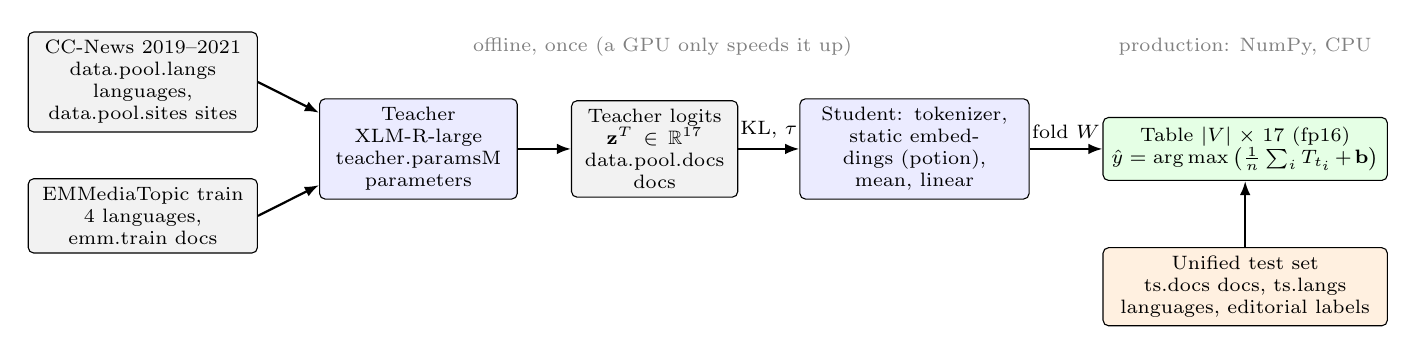
\begin{tikzpicture}[
  box/.style={draw, rounded corners=2pt, align=center, font=\scriptsize, inner sep=3pt, minimum height=8mm},
  data/.style={box, fill=gray!10},
  model/.style={box, fill=blue!8},
  prod/.style={box, fill=green!10},
  test/.style={box, fill=orange!12},
  arr/.style={-{Latex[length=1.8mm]}, thick},
  lab/.style={font=\scriptsize}]
  \node[data, text width=27mm] (cc)  at (1.4, 0.85)  {CC-News 2019--2021\\\val{data.pool.langs} languages, \val{data.pool.sites} sites};
  \node[data, text width=27mm] (emm) at (1.4,-0.85)  {EMMediaTopic train\\4 languages, \val{emm.train} docs};
  \node[model, text width=23mm] (t)  at (4.9, 0)     {Teacher\\XLM-R-large\\\val{teacher.params}M parameters};
  \node[data, text width=19mm] (soft) at (7.9, 0)    {Teacher logits\\$\mathbf{z}^{T}\in\mathbb{R}^{17}$\\\val{data.pool.docs} docs};
  \node[model, text width=27mm] (s)  at (11.2, 0)    {Student: tokenizer,\\static embeddings (potion),\\mean, linear};
  \node[prod, text width=34mm] (tab) at (15.4, 0)    {Table $|V|\times 17$ (fp16)\\$\hat{y}=\arg\max\big(\frac{1}{n}\sum_i T_{t_i}+\mathbf{b}\big)$};
  \node[test, text width=34mm] (ts) at (15.4, -1.75)  {Unified test set\\\val{ts.docs} docs, \val{ts.langs} languages, editorial labels};
  \draw[arr] (cc.east)  -- (t.160);
  \draw[arr] (emm.east) -- (t.200);
  \draw[arr] (t) -- (soft);
  \draw[arr] (soft) -- node[lab, above]{KL, $\tau$} (s);
  \draw[arr] (s) -- node[lab, above]{fold $W$} (tab);
  \draw[arr] (ts.north) -- (tab.south);
  \node[lab, text=gray] at (8.0, 1.3) {offline, once (a GPU only speeds it up)};
  \node[lab, text=gray] at (15.4, 1.3) {production: NumPy, CPU};
\end{tikzpicture}
\caption{StaticKD pipeline. The teacher labels an unlabeled news corpus once, offline. The student learns to imitate the teacher distribution, and its linear head is then folded into a token table, so inference only looks up and averages table rows. The final evaluation uses a test set whose labels do not come from the teacher.}
\label{fig:pipeline}
\end{figure*}

\subsection{Problem Formulation}
Given a news article $d$ in any language, consisting of its title and body truncated to the first 512 words as in~\cite{kuzman2025llm}, a model predicts one label $y\in\mathcal{Y}$ among the 17 top-level IPTC topics. The teacher $f_T$ outputs logits $\mathbf{z}^T(d)\in\mathbb{R}^{17}$. The goal is a student $f_S$ whose inference costs $O(n)$ additions for $n$ tokens, without matrix multiplication and without a deep learning library, and whose accuracy against independent labels is as close as possible to that of $f_T$.

\subsection{Distillation Data and Development Set}
EMMediaTopic 1.0~\cite{emmediatopic2025,kuzman2025llm} contains Catalan, Greek, Croatian, and Slovenian articles labeled by GPT-4o. Its training split (\val{emm.train} articles) is part of the distillation data. Its development split (\val{emm.dev} articles, median \val{emm.dev.words} words) was never used to train the teacher or the student and serves as the development set for choosing the recipe.

The multilingual CC-News corpus~\cite{cloversearch_ccnews} from the 2019--2021 archive was processed with the following steps.
\begin{enumerate}
  \item Keep only documents whose metadata language agrees with fastText language identification~\cite{joulin2017bag}.
  \item Take the title and body with at least 75 words (200 characters for ja, zh, th, my) and truncate to 512 words.
  \item Keep at most 150 documents per site.
  \item Form a held-out split by domain: all documents of some sites are set aside, at most 20\% per language.
  \item Add \val{data.ccextra.docs} documents from training sites only (at most 5,000 per language and 400 per site).
\end{enumerate}
The distillation data contain \val{data.pool.docs} documents in \val{data.pool.langs} languages from \val{data.pool.sites} sites, with a median of \val{data.pool.words} words. The held-out split is domain-disjoint within each language. A few multilingual sites (for example bbc.com) also appear in other languages of the distillation data, so their articles were removed. The remaining fidelity set has \val{data.heldout.strict} documents in \val{data.heldout.strict.langs} languages from \val{data.heldout.strict.sites} sites that never occur in the distillation data.

\subsection{Unified Test Set Construction}
\label{sec:testset}
The first source is CC-NEWS 2024--2026, sampled as one WARC file per month from January 2024 to August 2026 (32 files) of the Common Crawl CC-NEWS archive~\cite{commoncrawl2026ccnews}. From each page, the schema.org JSON-LD blocks~\cite{guha2016schema} of type \texttt{NewsArticle} and its subtypes were extracted, with the fields \texttt{articleSection}, \texttt{BreadcrumbList}, \texttt{inLanguage}, \texttt{datePublished}, \texttt{isAccessibleForFree}, and \texttt{articleBody}. The text comes from \texttt{articleBody} when it has at least 30 words and is otherwise extracted with Trafilatura~\cite{barbaresi2021trafilatura}. Sites that occur in the distillation data or in another evaluation set were removed, which leaves \val{ts.html_articles} articles from new sites.

The second source is public datasets. MasakhaNEWS~\cite{adelani2023masakhanews} and MN-DS~\cite{petukhova2023mnds} are labeled by humans. L3Cube-IndicNews (LDC split)~\cite{mirashi2023indicnews}, Bangla news~\cite{hossain2025banglanews}, IndoNews~\cite{indonews2021}, Amharic news~\cite{amharicnews2024}, and Swahili news~\cite{swahilinews2020} carry publisher categories. The last two were processed in the same way but were not selected during sampling, because MasakhaNEWS already filled their language cells with human labels. The second source holds \val{ts.ext_loaded} articles in total.

Section and category labels represent \emph{editorial topics}, that is, the decision of the newsroom about where an article belongs when it is published. These labels come from no model that reads the article text, so they are not circular with respect to the teacher. The only added step is translating section names onto the official IPTC Media Topic tree (\val{iptc.nodes} active nodes). Section names are normalized (case, diacritics) and mapped conservatively. A name is mapped only if the content usually found under that section belongs to one top-level topic. This gives \val{map.names} names mapped to \val{map.nodes} nodes. The table deliberately leaves \val{map.ambiguous} ambiguous names unmapped, for example \emph{tech}, which can be \emph{science and technology} or the information technology industry under \emph{economy}. Likewise, \emph{entertainment} can be \emph{arts} or \emph{lifestyle}, and \emph{terrorism} can be \emph{conflict} or \emph{crime}. Astrology sections are rejected. An automatic check verifies that every target node exists in the IPTC tree, is not retired, and has the target label as its level-1 ancestor. Articles whose sections map to different labels are rejected. MN-DS needs no mapping, because its labels already are IPTC topics. The mapping table was drafted with artificial intelligence assistance, and the first author reviewed all of its \val{map.review.total} rules (\val{map.names} mapped names and \val{map.review.other} ambiguous, language-specific, and rejecting rules) and accepted them without changes.

Quality and leakage filters are applied in order.
\begin{enumerate}
  \item Publication date on or after 1 January 2024 (CC-NEWS only).
  \item Not behind a paywall.
  \item Declared language agrees with fastText language identification when the language is supported.
  \item At least 75 words.
  \item Deduplication of uniform resource locators (URLs), identical texts, and near-duplicates (MinHash~\cite{broder1997resemblance}, Jaccard $\ge 0.7$~\cite{lee2022dedup}) across all sources.
  \item Contamination: an article is dropped when $\ge 30\%$ of its word 8-grams occur in any of about 300 thousand training or evaluation documents. This filter removed \val{ts.contam_removed} articles, mostly from MasakhaNEWS, which also draws on BBC.
\end{enumerate}

Sampling takes at most 50 articles per language $\times$ label cell, preferring human-labeled sources, then publisher categories, then JSON-LD sections. Languages with fewer than 30 articles are dropped. The number of articles per site is not capped, because most cells come from few sites and such a cap would discard data without adding diversity. The evaluation handles the dependence between articles of the same site with a site-cluster bootstrap, and Section~\ref{sec:res-acc} reports a sensitivity test with at most five articles per site.

The final test set contains \val{ts.docs} articles in \val{ts.langs} languages, with \val{ts.labels} labels and \val{ts.sites} sites or sources and a median of \val{ts.words} words. Of these, \val{ts.origin.human_annotation} articles (\val{ts.origin.human_annotation.pct}) carry human annotations, \val{ts.origin.publisher_category} (\val{ts.origin.publisher_category.pct}) publisher categories, and \val{ts.origin.publisher_section_jsonld} (\val{ts.origin.publisher_section_jsonld.pct}) JSON-LD sections. By the distillation data in their language, \val{ts.distil.tidak.langs} languages are entirely absent from the distillation data (for example ha, yo, ig, bn, pa), \val{ts.distil.sedikit.langs} have fewer than 500 documents, and \val{ts.distil.cukup.langs} have more. By site diversity, \val{ts.div.beragam.langs} languages have at least 10 effective sites, while \val{ts.div.satu.langs} languages come from practically one publisher. Table~\ref{tab:testset} summarizes the sources and Fig.~\ref{fig:testset} shows the language $\times$ label coverage.

\TabTestset

\begin{figure}[!t]
\centering
\includegraphics[width=\columnwidth]{figures/fig_testset_heatmap.pdf}
\caption{Articles in the unified test set per language and label (at most 50 per cell). The label origin in brackets is the dominant one for that language.}
\label{fig:testset}
\end{figure}

\subsection{Teacher and Distillation Labels}
The teacher is the IPTC classifier of~\cite{kuzman2025llm}, published as \url{classla/multilingual-IPTC-news-topic-classifier}. It is an XLM-RoBERTa-large model with \val{teacher.layers} layers, \val{teacher.params} million parameters, and inputs of at most 512 tokens. Its architecture limits the input to 512 XLM-R tokens. The 512-word input of \val{trunc.teacher.pct} of the test articles exceeds this limit, and for those articles the teacher reads about \val{trunc.teacher.words_kept} of \val{trunc.teacher.words_total} words (medians). For every distillation document the teacher produces a logit vector $\mathbf{z}^{T}(d)\in\mathbb{R}^{17}$, which is stored in full. Labeling ran once in fp16 on an NVIDIA RTX~4050 Laptop GPU (6~GB), with batches sorted by text length. On a fixed sample of \val{teacher.label_sample} documents the teacher labels \val{teacher.label_dps} documents per second, so the whole distillation set takes about \val{teacher.label_hours} GPU hours. The arg-max predictions of this re-run agree with the stored labels for \val{teacher.label_agree} of the documents. The teacher label distribution on CC-News is plausible (\emph{politics} \val{teacher.share.politics}, \emph{economy} \val{teacher.share.economy}, \emph{sport} \val{teacher.share.sport}, \emph{weather} \val{teacher.share.weather}), and its mean confidence per language ranges from \val{teacher.conf.min} to \val{teacher.conf.max}.

\subsection{The StaticKD Student}
A document $d$ is tokenized into $t_1,\dots,t_n$ with the potion-multilingual-128M Unigram tokenizer~\cite{tulkens2024model2vec}, which has \val{student.vocab} tokens. Special tokens are not used, unknown tokens are dropped, and the length is capped at 1,024 tokens. Averaging has no position limit, so the cap only bounds the cost. Only \val{trunc.statickd.pct} of the test articles exceed it. Each token has an embedding $\mathbf{e}_t\in\mathbb{R}^{\val{student.dim}}$, and
\begin{equation}
\mathbf{h}(d)=\frac{1}{n}\sum_{i=1}^{n}\mathbf{e}_{t_i},\qquad
\mathbf{z}^{S}(d)=W\,\mathrm{drop}(\mathbf{h}(d))+\mathbf{b},
\label{eq:student}
\end{equation}
with $W\in\mathbb{R}^{17\times 256}$ and dropout 0.1 during training. The embedding matrix $E$ is initialized from potion-multilingual, static embeddings for 101 languages distilled from BGE-M3~\cite{chen2024bgem3}.

The loss in \eqref{eq:kd} uses $p^{T}=\mathrm{softmax}(\mathbf{z}^{T}/\tau)$ and $p^{S}=\mathrm{softmax}(\mathbf{z}^{S}/\tau)$:
\begin{equation}
\mathcal{L}_{\mathrm{KD}}=\tau^{2}\,\mathrm{KL}\!\left(p^{T}\,\middle\|\,p^{S}\right),\qquad \tau=1 .
\label{eq:kd}
\end{equation}
$E$, $W$, and $\mathbf{b}$ are trained end to end. $E$ uses SparseAdam ($\eta=10^{-3}$), so only the rows of tokens present in a batch are updated, while $W$ and $\mathbf{b}$ use AdamW ($\eta=3\cdot 10^{-3}$, weight decay $10^{-4}$). The batch size is 64 and training runs for 6 epochs. As a cheap augmentation, each token of a training document is dropped with probability 0.2 at every step (token dropout), so that the model does not rely on a few keywords. Internal validation uses 3\% of the distillation data (\val{train.val_docs} documents), and the epoch with the highest arg-max agreement with the teacher is kept.

Because the classification head is linear, \eqref{eq:student} can be rewritten as
\begin{equation}
W\Big(\frac{1}{n}\sum_{i}\mathbf{e}_{t_i}\Big)+\mathbf{b}=\frac{1}{n}\sum_{i}T_{t_i}+\mathbf{b},
\label{eq:fold}
\end{equation}
with the table $T=EW^{\top}\in\mathbb{R}^{|V|\times 17}$. The production model consists only of $T$ (fp16), $\mathbf{b}$, and the tokenizer, and inference is tokenization, averaging table rows, and adding the bias. Averaging the logits of $K$ students trained with different seeds is likewise equal to the logits of a single student with table $\bar{T}=\frac{1}{K}\sum_k T^{(k)}$ and bias $\bar{\mathbf{b}}$, because \eqref{eq:fold} is linear in $T$. The final StaticKD model is the table ensemble of seeds 0, 1, and 2 ($K=3$), with \val{final.params} million parameters and a size of \val{final.size}~MB.

The internal structure of the Unigram tokenizer needs much more random-access memory (RAM) than the table itself (\val{final.table_mb}~MB). A compact variant shrinks that structure by removing token pieces that occur fewer than 10 times in the distillation corpus, keeping single characters. Its vocabulary has \val{compact.vocab} tokens and the model takes \val{compact.size}~MB. Table~\ref{tab:hparams} lists the hyperparameters of all models.

\TabHparams

\subsection{Baselines}
All baselines are trained on the same distillation data (\val{data.pool.docs} documents) with targets from the same teacher. fastText + KD~\cite{joulin2017bag} is trained on teacher arg-max labels with word tokens (plus character n-grams) or XLM-R subwords, together with a quantized variant (\texttt{.ftz}). As a reference equivalent to the labeled data available to~\cite{kuzman2025llm}, fastText is also trained only on the GPT-4o labels of the EMMediaTopic training split. TF-IDF + SVM + KD is the non-neural baseline of Kuzman and Ljube\v{s}i\'c (TF-IDF features with a support vector classifier), trained on teacher arg-max labels over XLM-R subwords. The hyperparameters of these non-transformer baselines were set once, as listed in Table~\ref{tab:hparams}, without a search. MiniLM-L6 + KD uses mMiniLMv2-L6-H384, distilled from XLM-R-large~\cite{wang2021minilmv2}, with the temperature $\tau\in\{1,2\}$ chosen on the development set. DistilmBERT + KD uses \texttt{distilbert-base-multilingual-cased}~\cite{sanh2019distilbert} with the same recipe. Both transformers read at most 256 tokens, which truncates \val{trunc.minilm_kd.pct} (MiniLM-L6) and \val{trunc.distilmbert_kd.pct} (DistilmBERT) of the test articles to about \val{trunc.minilm_kd.words_kept} and \val{trunc.distilmbert_kd.words_kept} words. Both are exported to ONNX fp32 for the CPU benchmark. The ONNX int8 teacher is a dynamic int8 quantized export of the teacher and is its fastest CPU configuration.

Sparse Distillation~\cite{ye2022sparse}, the closest prior work, was not reproduced in full. Two experiments of this study cover its core ideas. fastText + KD is a bag-of-n-grams model with averaging and a linear head, trained on teacher labels over the same transfer set. The random-initialization ablation (Section~\ref{sec:design}) trains the embedding table from scratch. What remains different is the hidden layers of the deep averaging network, the soft-logit targets, and the billion-parameter n-gram table designed for English. The frozen-embedding ablation, which trains only the linear head on top of potion, serves as an off-the-shelf Model2Vec baseline with a distilled head. The classifier trainer of the Model2Vec library was not run as a baseline. Its default configuration trains on hard labels and adds a 512-unit hidden layer. It also learns a weight per token. The ablations replace soft labels with hard labels and the linear head with a 512-unit hidden layer one at a time, and neither change differs significantly from the final recipe on the development or test set (Table~\ref{tab:ablation}). The two changes together and the learned token weights were not tested. A hidden layer also prevents folding the model into one table.

\subsection{Evaluation Protocol and Statistical Tests}
\label{sec:protocol}
The main metric is macro-F1 over the labels present in the reference, as in the evaluation code of~\cite{kuzman2025llm}, because the label distribution is imbalanced. The evaluation also reports accuracy, macro-F1 per language averaged over languages so that large languages do not dominate, and agreement with the teacher on the fidelity set. On editorial labels, macro-F1 reads as agreement between the predictions and the categorization of the publisher.

95\% confidence intervals come from a percentile bootstrap with 1,000 resamples. On the test set, the resampling unit is the site, or the source dataset when no URL is available (site-cluster bootstrap~\cite{field2007bootstrapping}). On the development set, the unit is the document. Two models on the same documents are compared with a paired (cluster) bootstrap with 2,000 resamples for $\Delta$macro-F1~\cite{koehn2004significance} and an exact McNemar test for accuracy~\cite{mcnemar1947}, with Holm correction~\cite{holm1979} within each set. Each ablation variant uses five seeds, and the final recipe uses ten. Differences between variants are tested with Welch tests at the seed level, Holm-corrected. Whether a difference holds consistently across languages is tested with a Wilcoxon signed-rank test on per-language macro-F1 and accuracy~\cite{dror2018hitchhiker}. Subgroup analyses cover label origin, region, the amount of distillation data of the language, site diversity, script, language, and label. Calibration is measured with the expected calibration error (ECE, 15 bins)~\cite{guo2017calibration}.

\subsection{Efficiency Protocol}
\label{sec:effprotocol}
The benchmark runs on CPU only, with the GPU hidden. Each model runs in a fresh process, and the thread count is pinned in every library (OMP, MKL, OpenBLAS, ONNX Runtime, \texttt{tokenizers}). Latency is measured with one article per call, as in a streaming setting (p50 and p95), and throughput with batches of 64, or 8 for transformers. Model RAM is the increase in resident set size after loading the model. The text sample is drawn at random from the unified test set and is the same for every model: \val{eff.teacher.n_latency} latency and \val{eff.teacher.n_throughput} throughput documents for the teacher and the transformers, and \val{eff.statickd.n_latency} and \val{eff.statickd.n_throughput} for the light models. All models are measured in one session on an idle machine. StaticKD reads up to 1,024 tokens per article while the teacher stops at 512, so the speed comparison does not favor StaticKD.

The machine is a laptop with an Intel Core Ultra~7 155H, 31~GB of RAM, and Windows~11. This CPU is hybrid, with 6 P-cores, 8 slower E-cores, and 2 low-power E-cores. Without pinning, the operating system moves threads to the slow cores. Each process is therefore pinned to physical P-cores (logical CPU 0 for one core; logical CPUs 0, 10, 12, and 14 for four cores), which approximates a small server with uniform cores.

\subsection{Experimental Design and Implementation Details}
\label{sec:design}
Table~\ref{tab:ablation} lists all \val{runs.total} StaticKD runs. Each ablation variant changes one factor of the final recipe: hard labels instead of soft labels; EMMediaTopic data only (4 languages, 10 epochs); 130 thousand documents without the extra CC-News data; random initialization with the same standard deviation as potion; frozen embeddings; no token dropout; a 512-unit multilayer perceptron (MLP) head; and $\tau\in\{0.5,\,2,\,4\}$. Four exploratory variants were also tested: bigram hashing ($2^{21}$ buckets), idf$^{0.5}$-weighted pooling, document weights from teacher confidence, and an additional cross-entropy term on the GPT-4o labels. One StaticKD run takes \val{train.seconds} minutes on average on the same GPU. The implementation uses Python~3.12, NumPy~2.5, PyTorch~2.6, transformers~5.17, \texttt{tokenizers}~0.23, ONNX Runtime~1.30, scikit-learn~1.9, and fastText~0.9.2. The seed, library versions, and training history of every run are stored with the model.


\section{Results}
\label{sec:results}
\subsection{Accuracy of All Models (RQ2)}
\label{sec:res-acc}
\TabMain
Table~\ref{tab:main} gives the main results. On the unified test set the teacher reaches a macro-F1 of \val{teacher.test.macro} [\val{teacher.test.ci}] and an accuracy of \val{teacher.test.acc}. This is far below its development score (\val{teacher.dev.macro}), because the test set covers languages, sources, and a period the teacher has never seen. StaticKD reaches a macro-F1 of \val{statickd.test.macro} [\val{statickd.test.ci}] and an accuracy of \val{statickd.test.acc}, which is \val{statickd.test.pct_teacher} of the teacher macro-F1. On the development set StaticKD keeps \val{statickd.dev.pct_teacher} of the teacher macro-F1 (\val{statickd.dev.macro} against \val{teacher.dev.macro}), and its agreement with the teacher over the \val{data.heldout.strict.langs} held-out languages is \val{statickd.heldout.acc}. A single student without ensembling reaches \val{single.test_macro.mean} $\pm$ \val{single.test_macro.sd} on the test set and \val{single.dev_macro.mean} $\pm$ \val{single.dev_macro.sd} on the development set (10 seeds).

Among the small distilled transformers, MiniLM-L6 (\val{minilm_kd.test.macro}), which starts from a distillation of XLM-R-large, lies between StaticKD and the teacher. DistilmBERT (\val{distilmbert_kd.test.macro}) is on par with StaticKD while being much more expensive. The two baselines of similar cost, fastText + KD and TF-IDF + SVM + KD, fall below StaticKD. fastText trained only on the GPT-4o labels of four languages fails outside its training languages, with a test macro-F1 of \val{ft_gpt_subword.test.macro} against \val{ft_gpt_subword.dev.macro} on the development set.

\TabSig
Table~\ref{tab:sig} reports paired tests with $\Delta$ = StaticKD $-$ comparison model on the test set. Against the teacher, $\Delta$macro-F1 is \val{sig.test.teacher.delta} [\val{sig.test.teacher.ci}] ($p$ \val{sig.test.teacher.p}), and against MiniLM-L6 it is \val{sig.test.minilm_kd.delta} [\val{sig.test.minilm_kd.ci}] ($p$ \val{sig.test.minilm_kd.p}). The difference to DistilmBERT, \val{sig.test.distilmbert_kd.delta} [\val{sig.test.distilmbert_kd.ci}], is not significant ($p$ \val{sig.test.distilmbert_kd.p}). StaticKD is correct on more test documents than DistilmBERT (McNemar $p$ \val{sig.test.distilmbert_kd.pm}), but the McNemar test treats documents as independent and ignores the dependence between articles of the same site. StaticKD outperforms the quantized fastText + KD by \val{sig.test.ft_kd_subword_q.delta} [\val{sig.test.ft_kd_subword_q.ci}] ($p$ \val{sig.test.ft_kd_subword_q.p}) and TF-IDF + SVM by \val{sig.test.tfidf_svm_kd.delta} [\val{sig.test.tfidf_svm_kd.ci}] ($p$ \val{sig.test.tfidf_svm_kd.p}).

These two advantages differ in strength when examined per language. StaticKD has a higher macro-F1 than fastText + KD in \val{lang.static_better_macro.ft_kd_subword_q} of \val{lang.n} languages (Wilcoxon $p$ \val{lang.wilcoxon_macro.ft_kd_subword_q.p}) and a higher accuracy in \val{lang.static_better.ft_kd_subword_q} (Wilcoxon $p$ \val{lang.wilcoxon.ft_kd_subword_q.p}). Against TF-IDF + SVM it has a higher macro-F1 in \val{lang.static_better_macro.tfidf_svm_kd} of \val{lang.n} languages (Wilcoxon $p$ \val{lang.wilcoxon_macro.tfidf_svm_kd.p}), but a higher accuracy in only \val{lang.static_better.tfidf_svm_kd} and a lower accuracy in \val{lang.static_worse.tfidf_svm_kd} (Wilcoxon $p$ \val{lang.wilcoxon.tfidf_svm_kd.p}). The advantage over TF-IDF + SVM is thus consistent across languages on the main metric, while the per-language accuracies of the two models are close. Against DistilmBERT neither metric differs consistently across languages (Wilcoxon $p$ \val{lang.wilcoxon_macro.distilmbert_kd.p} for macro-F1 and \val{lang.wilcoxon.distilmbert_kd.p} for accuracy). StaticKD beats the teacher in only \val{lang.static_better.teacher} of \val{lang.n} languages (Wilcoxon $p$ \val{lang.wilcoxon.teacher.p}).

By label origin (Table~\ref{tab:groups}, Fig.~\ref{fig:groups}), StaticKD retains \val{grp.label_origin.publishersection.pct} of the teacher score on articles with JSON-LD section labels, \val{grp.label_origin.publishercategor.pct} on publisher categories, and \val{grp.label_origin.humanannotation.pct} on human annotations. By the distillation data of the language, it retains \val{grp.distil_tier.cukup.pct} in languages with sufficient data, \val{grp.distil_tier.sedikit.pct} in languages with little data, and \val{grp.distil_tier.tidakada.pct} in languages with no distillation data at all. On a subset with at most five articles per site and cell (\val{sens.n} articles), the model ranking is \val{sens.rank_same} relative to the full test set (StaticKD \val{sens.statickd}, teacher \val{sens.teacher}).

\TabGroups

Table~\ref{tab:sources} splits the test set by source. On MN-DS, the only source annotated directly with IPTC topics, StaticKD keeps \val{src.mnds.pct} of the teacher score (\val{src.mnds.statickd} against \val{src.mnds.teacher}), and the teacher itself reaches its lowest macro-F1 of all sources there. The lowest retention is on MasakhaNEWS (\val{src.masakhanews.pct}), whose human labels follow a non-IPTC scheme and most of whose African languages are absent from the distillation data. Bangla is also absent from the distillation data. On Bangla news, fastText + KD and TF-IDF + SVM collapse to \val{src.bangla_plos.ft_kd_subword_q} and \val{src.bangla_plos.tfidf_svm_kd}, while StaticKD reaches \val{src.bangla_plos.statickd}. This gap shows the cross-lingual transfer that baselines without pre-trained embeddings lack.

\TabSources

\begin{figure*}[!t]
\centering
\includegraphics[width=0.78\textwidth]{figures/fig_groups.pdf}
\caption{Test macro-F1 by label origin (left) and by the amount of distillation data in the language of the article (right).}
\label{fig:groups}
\end{figure*}

\subsection{Validity of the Editorial Labels}
\label{sec:res-validity}
Section and category labels record newsroom decisions, so the question is whether they agree with human labels in the same language.

All English cells of the test set are filled with human-labeled sources. As a comparison within the same language, a separate sample of \val{valid.en.silver.n} English CC-NEWS articles with JSON-LD section labels was therefore drawn from \val{valid.en.silver.sites} sites outside the test set, at most 50 per label. The teacher reaches an accuracy of \val{valid.en.silver.acc} on the section labels (macro-F1 \val{valid.en.silver.macro}) and \val{valid.en.human.acc} on the MN-DS and MasakhaNEWS human labels (macro-F1 \val{valid.en.human.macro}). Accuracy on section labels is higher for \val{valid.en.labels_higher} of the 17 labels (Wilcoxon $p$ \val{valid.en.wilcoxon.p}), and the ranking of label difficulty correlates between the two label types ($\rho=\val{valid.en.label_rho}$, $p$ \val{valid.en.label_rho.p}). The hard labels, \emph{society}, \emph{human interest}, and \emph{religion}, are hard under both.

French offers a second comparison inside the test set. The teacher reaches an accuracy of \val{valid.fr.rubrik.acc} on \val{valid.fr.rubrik.n} articles with section labels and \val{valid.fr.anotasi.acc} on \val{valid.fr.anotasi.n} human-labeled MasakhaNEWS articles.

A last check looks at each source category, restricted to languages covered by XLM-R pre-training. The median agreement of the teacher with the mapped label per category is \val{mapcheck.masakhanews.median} for MasakhaNEWS, \val{mapcheck.mnds.median} for MN-DS, \val{mapcheck.l3cube_indic.median} for L3Cube, and \val{mapcheck.ccnews_jsonld.median} for CC-NEWS sections. The lowest agreement occurs for source categories that are broader than their IPTC target. For example, only \val{mapcheck.masakha_politics} of MasakhaNEWS \emph{politics} articles are predicted as \emph{politics}, with \val{mapcheck.masakha_politics.alt} as the main alternative. Agreement is also low for labels whose boundaries are unclear even to human annotators, such as \emph{society} in MN-DS, in line with the low inter-annotator agreement reported for that label~\cite{kuzman2025llm}. Such mismatches reflect differences between the category scheme of a source and IPTC. Since every model is scored against the same labels, comparisons between models are unaffected, and absolute scores read as agreement with the editorial categorization.

\subsection{Ablation, Temperature, and Ensembling (RQ3)}
\TabAblation
\TabAblationGroups
Table~\ref{tab:ablation} gives the contribution of each component with five seeds per variant. Multilingual distillation data matter most. Distilling on EMMediaTopic alone (4 languages) lowers the test macro-F1 by \val{abl.emm_only.test_macro.delta} and the held-out agreement by \val{abl.emm_only.heldout_acc.delta}. Random initialization changes the test macro-F1 by \val{abl.random_init.test_macro.delta} ($p$ \val{abl.random_init.test_macro.p}), so the cross-lingually aligned embeddings account for a large share of the accuracy.

Freezing the embeddings and training only the linear head on top of potion lowers the development score by \val{abl.frozen.dev_macro.delta} ($p$ \val{abl.frozen.dev_macro.p}) and the held-out agreement by \val{abl.frozen.heldout_acc.delta} ($p$ \val{abl.frozen.heldout_acc.p}). On the test set the same variant raises macro-F1 by \val{abl.frozen.test_macro.delta} ($p$ \val{abl.frozen.test_macro.p}). Table~\ref{tab:ablation-groups} shows that this gain comes from languages with little distillation data (\val{ablgrp.frozen.sedikit.delta}) and with none (\val{ablgrp.frozen.tidakada.delta}). In data-rich languages the frozen embeddings are weaker (\val{ablgrp.frozen.cukup.delta}).

Hard teacher labels change the test macro-F1 by \val{abl.hard.test_macro.delta} ($p$ \val{abl.hard.test_macro.p}) and the development score by \val{abl.hard.dev_macro.delta} ($p$ \val{abl.hard.dev_macro.p}), so they do not differ from soft labels. Reducing the data to 130 thousand documents changes the test macro-F1 by \val{abl.data130k.test_macro.delta} ($p$ \val{abl.data130k.test_macro.p}), removing token dropout by \val{abl.no_tdrop.test_macro.delta} ($p$ \val{abl.no_tdrop.test_macro.p}), and an MLP head that cannot be folded by \val{abl.mlp.test_macro.delta} ($p$ \val{abl.mlp.test_macro.p}).

Fig.~\ref{fig:temperature} shows the effect of temperature. Compared with $\tau=1$, the common choice $\tau=2$~\cite{hinton2015distilling} lowers the held-out agreement by \val{abl.tau2.heldout_acc.delta} ($p$ \val{abl.tau2.heldout_acc.p}). Its changes on the test macro-F1 (\val{abl.tau2.test_macro.delta}, $p$ \val{abl.tau2.test_macro.p}) and on the development set (\val{abl.tau2.dev_macro.delta}, $p$ \val{abl.tau2.dev_macro.p}) are not significant. With $\tau=4$ all three metrics drop, and on the test set the drop is \val{abl.tau4.test_macro.delta} ($p$ \val{abl.tau4.test_macro.p}). None of the four exploratory variants improves the test set: bigram hashing \val{abl.bigram.test_macro.delta}, idf pooling \val{abl.idf.test_macro.delta}, confidence weights \val{abl.conf.test_macro.delta}, and cross-entropy on GPT-4o labels \val{abl.gpt_ce.test_macro.delta}.

Growing the ensemble from one to three seeds moves the test macro-F1 from \val{ens.k1.test_macro} to \val{ens.k3.test_macro} and the held-out agreement from \val{ens.k1.heldout_acc} to \val{ens.k3.heldout_acc} (Fig.~\ref{fig:ensemble}). Ten seeds give \val{ens.k10.test_macro}. The gain is small, but it costs nothing at inference time because every ensemble size is still one table.

\begin{figure*}[!t]
\centering
\includegraphics[width=0.9\textwidth]{figures/fig_temperature.pdf}
\caption{Effect of the distillation temperature. Each dot is one seed; the line connects the means.}
\label{fig:temperature}
\end{figure*}

\begin{figure}[!t]
\centering
\includegraphics[width=0.85\columnwidth]{figures/fig_ensemble_size.pdf}
\caption{Effect of the table ensemble size (mean $\pm$ standard deviation over seed combinations).}
\label{fig:ensemble}
\end{figure}

\subsection{CPU Efficiency (RQ1)}
\label{sec:res-eff}
\TabEff
Table~\ref{tab:eff} and Figs.~\ref{fig:tradeoff} and~\ref{fig:latency} show the efficiency of all models. In PyTorch fp32 the teacher needs \val{eff.teacher.latency_ms_p50_1c}~ms per article on one core, with a throughput of \val{eff.teacher.docs_per_sec_1c} articles per second. Its best CPU configuration, ONNX int8, needs \val{eff.teacher_onnx_int8.latency_ms_p50_1c}~ms with a throughput of \val{eff.teacher_onnx_int8.docs_per_sec_1c} articles per second. Classifying one million articles per day would take \val{eff.teacher_onnx_int8.cores1M} cores (ONNX int8) to \val{eff.teacher.cores1M} cores (PyTorch) for this step alone.

StaticKD needs \val{eff.statickd.latency_ms_p50_1c}~ms per article and processes \val{eff.statickd.docs_per_sec_1c} articles per second per core. This is about \val{eff.statickd.speedup_onnx} times faster than the ONNX int8 teacher, \val{eff.statickd.speedup_pt} times faster than the PyTorch teacher, and \val{eff.speed_vs_minilm} times faster than MiniLM-L6. Its file is \val{eff.size_ratio_onnx} times smaller than the ONNX int8 teacher, and one million articles per day need \val{eff.statickd.cores1M} cores. Its model RAM is \val{eff.statickd.ram}~MB, mostly for the tokenizer structure. The compact variant reduces it to \val{eff.statickd_compact.ram}~MB. With one thread, tokenization (\val{prof.statickd.tokens} tokens per article on average) takes \val{prof.statickd.tokshare} of the prediction time, while table pooling alone runs at \val{prof.statickd.pool_dps} articles per second. The speed limit of StaticKD is thus set by the tokenizer implementation.

StaticKD is not the fastest model in the table. The quantized fastText + KD is slightly faster (\val{eff.ft_kd_subword_q.docs_per_sec_1c} articles per second), smaller (\val{eff.ft_kd_subword_q.size}~MB), and uses less RAM (\val{eff.ft_kd_subword_q.ram}~MB), but its test macro-F1 is \val{ft_kd_subword_q.test.macro} against \val{statickd.test.macro} for StaticKD. Among the models with comparable latency, namely StaticKD, its compact variant, fastText, and TF-IDF + SVM, StaticKD is the most accurate (Fig.~\ref{fig:tradeoff}).

\begin{figure}[!t]
\centering
\includegraphics[width=\columnwidth]{figures/fig_tradeoff.pdf}
\caption{Test macro-F1 on the unified test set against single-core CPU throughput (log scale).}
\label{fig:tradeoff}
\end{figure}

\begin{figure*}[!t]
\centering
\includegraphics[width=0.9\textwidth]{figures/fig_latency_ram_size.pdf}
\caption{Latency per article, model RAM, and file size (log scale).}
\label{fig:latency}
\end{figure*}

\subsection{Analysis by Language and Label (RQ4)}
\TabFactors
The median per-language accuracy gap between StaticKD and the teacher is \val{lang.gap.median} (Fig.~\ref{fig:lang}). On the held-out set (\val{fac.langs} languages with at least 20 documents), the agreement of StaticKD correlates with the log amount of distillation data ($\rho=\val{fac.data.rho}$, $p$ \val{fac.data.p}) and with teacher confidence ($\rho=\val{fac.conf.rho}$, $p$ \val{fac.conf.p}), but does not differ across scripts (Kruskal--Wallis $H=\val{fac.kw.H}$, $p$ \val{fac.kw.p}; Table~\ref{tab:factors}). On languages outside XLM-R pre-training that are also absent from the distillation data (\val{lang.outxlmr.langs}), StaticKD reaches a mean accuracy of only \val{lang.outxlmr.static_acc}, while the teacher reaches \val{lang.outxlmr.teacher_acc}.

In \val{lang.vlowcov.n} languages (\val{lang.vlowcov.langs}), fewer than half of the token occurrences belong to tokens seen at least 10 times in the distillation data (at most \val{lang.vlowcov.cov_max}). StaticKD still reaches a mean accuracy of \val{lang.vlowcov.static_acc} in these languages (teacher \val{lang.vlowcov.teacher_acc}). The compact variant removes those tokens from the tokenizer, and its accuracy in these languages falls to \val{lang.vlowcov.compact_acc}. In the remaining languages the compact variant reaches \val{lang.restcov.compact_acc} against \val{lang.restcov.static_acc} for the full StaticKD. Section~\ref{sec:discussion} discusses the mechanism behind this pattern.

\begin{figure*}[!t]
\centering
\includegraphics[width=0.9\textwidth]{figures/fig_per_language.pdf}
\caption{Left: StaticKD accuracy against teacher accuracy per test language (color shows the distillation data of the language, size the number of articles). Right: held-out agreement per language against the amount of distillation data for StaticKD and fastText + KD.}
\label{fig:lang}
\end{figure*}

Per label (Fig.~\ref{fig:label}), the hardest labels for StaticKD are \val{label.hardest}, and the easiest are \val{label.easiest}. The largest gaps to the teacher occur for \val{label.biggest_gap}, and the most frequent confusions are \val{label.top_confusions}.

\begin{figure*}[!t]
\centering
\includegraphics[width=0.9\textwidth]{figures/fig_per_label.pdf}
\caption{F1 per label on the test set (left) and the StaticKD confusion matrix normalized per reference label (right).}
\label{fig:label}
\end{figure*}

\subsection{Calibration and Cascade Mode}
\TabCascade
The ECE of StaticKD is \val{ece.statickd.dev} on the development set and \val{ece.statickd.test} on the test set, lower than that of the teacher (\val{ece.teacher.dev} and \val{ece.teacher.test}). Both models become overconfident on the test set, which lies outside the training distribution (Fig.~\ref{fig:calib}). In cascade mode, StaticKD decides the articles on which its confidence is at least $\theta$ and sends the rest to the teacher (Table~\ref{tab:cascade}). With $\theta=0.8$, StaticKD decides \val{casc.08.coverage} of the articles with an accuracy of \val{casc.08.acc_covered}. The cascade reaches an overall accuracy of \val{casc.08.accuracy} and a macro-F1 of \val{casc.08.macro_f1}, against \val{casc.101.accuracy} and \val{casc.101.macro_f1} for the teacher alone, at an effective throughput of \val{casc.08.docs_per_sec} articles per second per core against \val{casc.101.docs_per_sec}. Sending about two fifths of the articles to the teacher is enough for the cascade to match the teacher accuracy.

\begin{figure}[!t]
\centering
\includegraphics[width=0.8\columnwidth]{figures/fig_calibration.pdf}
\caption{Reliability diagram of StaticKD on the development and test sets.}
\label{fig:calib}
\end{figure}


\section{Discussion}
\label{sec:discussion}
StaticKD keeps \val{statickd.test.pct_teacher} of the teacher macro-F1 on the unified test set and \val{statickd.dev.pct_teacher} on the development set, at an inference cost two to three orders of magnitude lower (\val{eff.statickd.speedup_onnx}$\times$ against ONNX int8 and \val{eff.statickd.speedup_pt}$\times$ against PyTorch). This agrees with the finding that order-free representations are already competitive for topic classification~\cite{galke2022bow}. Names of institutions, sports terms, and medical vocabulary carry most of the topic signal. The remaining gap concentrates in two places. The first is labels whose vocabulary overlaps with other topics. The largest gaps to the teacher occur for \val{label.biggest_gap}. The hardest labels for StaticKD, given here with their F1, are \val{label.hardest}. They are also among the hardest for the teacher. \emph{Society} and \emph{human interest} are known to be difficult for human annotators as well~\cite{kuzman2025llm}. The second is languages that are underrepresented in the distillation data. StaticKD reaches \val{grp.distil_tier.cukup.pct} of the teacher score in languages with sufficient distillation data but only \val{grp.distil_tier.tidakada.pct} in languages without any.

With the same distillation data, MiniLM-L6 closes part of this gap (StaticKD $-$ MiniLM \val{sig.test.minilm_kd.delta}, $p$ \val{sig.test.minilm_kd.p}), whereas DistilmBERT does not (\val{sig.test.distilmbert_kd.delta}, $p$ \val{sig.test.distilmbert_kd.p}). Both cost one to two orders of magnitude more than StaticKD. MiniLM comes from a distillation of XLM-R-large and DistilmBERT from mBERT, which suggests that the quality of the initial multilingual representation matters more than the number of layers.

The ablations show where the knowledge of the student comes from (RQ3). The largest source is the multilingual distillation data labeled by the teacher. Without it the test macro-F1 drops by \val{abl.emm_only.test_macro.delta}, consistent with Sparse Distillation~\cite{ye2022sparse}, which also relies on a large transfer set. The cross-lingually aligned initialization comes next, and the compact variant gives the most direct evidence for it. In Indian languages that hardly occur in the distillation data (for example bn, pa, or), most tokens are never updated during training and keep their initial potion embeddings. StaticKD still classifies these languages with a mean accuracy of \val{lang.vlowcov.static_acc}, yet the accuracy falls to \val{lang.vlowcov.compact_acc} once the tokenizer pruning removes those tokens. Transfer to languages without data is therefore carried by embedding rows that were never trained but live in the same space as the trained rows, so the linear head learned on data-rich languages applies to them too.

The frozen-embedding ablation shows the other side of the same mechanism. Fine-tuning moves the embeddings of tokens from languages in the distillation data and improves in-distribution fit. Freezing them lowers the development score by \val{abl.frozen.dev_macro.delta}. Tokens of other languages stay in the original potion space, where the head that adapted to the moved space fits them less well. In languages with no or little distillation data, frozen embeddings are better by \val{ablgrp.frozen.tidakada.delta} and \val{ablgrp.frozen.sedikit.delta}. This is representation drift caused by fine-tuning part of the vocabulary. The final recipe keeps fine-tuning because the recipe was selected on a development set in the training languages. For deployments that target languages without distillation data, frozen embeddings or a regularizer that keeps the embeddings close to potion are the safer choice, and both still fold into a table.

Soft labels, by contrast, add little or nothing. Hard teacher labels do not differ significantly from soft labels at $\tau=1$ (development \val{abl.hard.dev_macro.delta}, test \val{abl.hard.test_macro.delta}). Raising the temperature to $\tau=2$ lowers the held-out agreement without a significant change on the test set, and $\tau=4$ lowers every metric. This pattern fits the capacity-gap literature~\cite{zhang2025law,wang2026rckd}. A plausible explanation is that one linear layer over averaged embeddings cannot represent the inter-class structure in the tail of the teacher distribution (dark knowledge)~\cite{zhao2022dkd}. A sharp distribution ($\tau=1$) or hard labels give an attainable target, whereas a high $\tau$ asks the student to imitate a distribution shape beyond its capacity. For very-low-capacity students, effort is better spent on the coverage of the transfer set (languages, sites, topics) and on aligned initialization than on shaping the soft labels.

Per-language performance is driven mainly by how well a language is represented in the distillation and pre-training data, not by its script (Kruskal--Wallis $p$ \val{fac.kw.p}). The weakest languages are African languages outside XLM-R pre-training that are also missing from the distillation data (\val{lang.outxlmr.langs}). The teacher still reaches an accuracy of \val{lang.outxlmr.teacher_acc} on them, perhaps thanks to subwords shared with other languages and to sentence context, while StaticKD reaches only \val{lang.outxlmr.static_acc}. The cheapest fix needs no change of architecture. News in these languages can simply be added to the transfer set and labeled by the teacher. The data ablation and the correlation between agreement and the amount of data ($\rho=\val{fac.data.rho}$) support this step.

Some variants move agreement with the teacher and accuracy on editorial labels in opposite directions. Frozen embeddings lower the held-out agreement (\val{abl.frozen.heldout_acc.delta}) but raise the test macro-F1 (\val{abl.frozen.test_macro.delta}). Cutting the data to 130 thousand documents lowers the agreement (\val{abl.data130k.heldout_acc.delta}) without a significant change on the test set (\val{abl.data130k.test_macro.delta}). In line with~\cite{stanton2021kd}, students should be selected with labels that do not come from the teacher and with test data outside the training distribution, not with fidelity alone.

Test scores should be read according to the nature of the labels. Two thirds of the labels are editorial topics, the place where the newsroom put an article, translated to IPTC. An article about a criminal case involving an athlete can rightly sit in a sports section while a model labels it \emph{crime}. Both answers are plausible under IPTC, which allows several topics per article. Absolute scores on editorial labels thus measure agreement with the categorization of publishers. Comparisons between models remain fair because all models are scored against the same labels, and the model ranking does not change on the subset with capped site counts.

Compared with Sparse Distillation~\cite{ye2022sparse}, StaticKD replaces an n-gram table trained from scratch with pre-trained multilingual embeddings folded into 17 logits per token. The model becomes far smaller and transfers to languages that are missing from the transfer set. Inference is the recurring cost in a news pipeline, since every incoming article is classified, and one million articles per day need \val{eff.teacher_onnx_int8.cores1M} cores with the ONNX int8 teacher against \val{eff.statickd.cores1M} with StaticKD (Section~\ref{sec:res-eff}). Int8 quantization of the teacher only gives a constant-factor speed-up.

For a real-time pipeline on servers without a GPU, StaticKD processes one million articles per day with \val{eff.statickd.cores1M} cores, a \val{final.size}~MB file, and \texttt{numpy} and \texttt{tokenizers} as its only dependencies. Its probabilities are better calibrated than those of the teacher (test ECE \val{ece.statickd.test} against \val{ece.teacher.test}), which makes a cascade possible. With $\theta=0.8$, the cascade accuracy (\val{casc.08.accuracy}) equals that of the teacher alone (\val{casc.101.accuracy}) at \val{casc.08.docs_per_sec} articles per second per core, against \val{eff.teacher_onnx_int8.docs_per_sec_1c} for the teacher alone. This mode suits batch jobs that need teacher-level accuracy. The compact variant lowers RAM but is only advisable when all target languages are covered by the distillation data.


\section{Limitations}
\label{sec:limitations}
Of the test articles, \val{ts.origin.publisher_section_jsonld.pct} carry JSON-LD section labels and \val{ts.origin.publisher_category.pct} publisher categories. These labels are editorial topics. Section conventions differ between publishers, and one section reflects one editorial view of an article that may cover several topics. The mapping table is conservative, validated against the IPTC tree, and reviewed by the first author, but the articles were not re-annotated by humans. Absolute scores on these labels therefore measure agreement with the categorization of publishers, especially for labels with unclear boundaries (\emph{society}, \emph{human interest}, \emph{lifestyle}).

MasakhaNEWS labels were assigned by human annotators under their own scheme and then mapped to IPTC. Only MN-DS is annotated directly with IPTC topics, and it is English only. The multilingual IPTC test set of Kuzman and Ljube\v{s}i\'c~\cite{kuzman2025llm} is not public, so it was not available for this study.

Label coverage per language is uneven, with a median of \val{ts.lang_labels.median} labels per language, and the African languages cover only four or five broad topics. Macro-F1 is computed over the labels present, so per-language scores are not directly comparable between languages with different label coverage. Publisher diversity is also limited for some languages: \val{ts.div.satu.langs} languages come from practically one publisher, namely BBC/VOA for the African languages, L3Cube for the Indian languages, and a single site for several CC-NEWS languages. Claims for these languages are limited to those publishers, and the site-cluster bootstrap widens their confidence intervals accordingly.

The teacher bounds the student from above, and its errors and biases are copied. The fidelity set measures similarity to the teacher, not correctness.

The hyperparameters of fastText and TF-IDF + SVM were set once without a search, whereas the StaticKD recipe was selected from \val{runs.total} runs on the development set. This unequal tuning budget may widen the accuracy gap to these two baselines. The classifier trainer of the Model2Vec library was not run as a baseline, and only its components were tested separately as ablations. MiniLM-L6 and DistilmBERT were trained and evaluated with at most 256 tokens and therefore see less than half of most test articles, so their accuracy may be underestimated.

The benchmark ran on one machine in one session, with \val{eff.teacher.n_latency} latency documents for the teacher and the transformers. Absolute numbers on a server will differ and the latency sample of the heavy models is small, but ratios between models measured under the same protocol remain informative.

StaticKD is much less accurate on African languages that are absent from both the distillation data and pre-training (Section~\ref{sec:discussion}). Used as a topic filter, it could misclassify or drop news in these languages more often. Before deployment, accuracy should be monitored per language, and low-confidence articles should be routed to the teacher through the cascade mode.

The study covers only top-level IPTC labels and single-label classification. Deeper levels and multi-topic articles remain untested.


\section{Conclusion}
\label{sec:conclusion}
This study measured the CPU cost of the open multilingual IPTC classifier and showed that it can be cut by two to three orders of magnitude while keeping most of its accuracy. StaticKD distills the XLM-R-large teacher into a table of 17 logits per token, initialized from multilingual static embeddings and trained on \val{data.pool.docs} teacher-labeled articles in \val{data.pool.langs} languages. On a unified test set of \val{ts.docs} articles in \val{ts.langs} languages, with labels that do not come from the teacher, StaticKD reaches a macro-F1 of \val{statickd.test.macro}, or \val{statickd.test.pct_teacher} of the teacher. It processes \val{eff.statickd.docs_per_sec_1c} articles per second per CPU core, about \val{eff.statickd.speedup_onnx} times the speed of the ONNX int8 teacher, with a \val{final.size}~MB model that needs no deep learning library.

The accuracy of this very-low-capacity student comes mainly from the multilingual transfer set and from cross-lingually aligned embeddings. Soft labels are no better than hard labels, $\tau=4$ lowers every metric, and an ensemble of seeds folds into one table at no cost. Fine-tuning the embeddings raises accuracy in languages present in the distillation data but lowers it in languages without distillation data, because transfer to those languages is carried by pre-trained embeddings that are never updated. The test set, with editorial labels mapped onto the IPTC tree, contamination control, and site-cluster bootstrap, can be reused to evaluate other IPTC classifiers.

Several directions follow from these results. The transfer set should be extended to the weak languages, especially the African languages outside XLM-R pre-training. A fine-tuning regularizer that keeps embeddings close to the pre-trained space could give in-distribution accuracy and cross-lingual transfer at the same time. Tokenization takes \val{prof.statickd.tokshare} of the inference time, so a faster tokenizer, for instance a direct word-to-table lookup, is the next source of speed. Any pruning of the vocabulary has to keep cross-lingual tokens. Cheap non-linear heads with quantized embeddings, hierarchical classification into IPTC level 2, multi-label classification, and human IPTC annotation of a multilingual sample of the test set remain open.


\section*{Code, Model, and Data Availability}
The code for data collection, test-set construction, teacher labeling, training, evaluation, and benchmarking, together with a notebook that reproduces every number, table, and figure of this paper, is available at \todo{GitHub URL and Zenodo DOI}. The StaticKD models are available at \todo{Hugging Face URL}. The test set is released as a manifest of article URLs or IDs, labels, label origins, and text hashes, with a reconstruction script. Article texts are not redistributed because of publisher copyright and the licenses of the source datasets. The section-to-IPTC mapping table is released with the code. EMMediaTopic is available from the CLARIN.SI repository~\cite{emmediatopic2025}. Table~\ref{tab:license} lists the licenses of the assets used and released in this study.

\TabLicense


\section*{Acknowledgment}
The authors thank the Department of Informatics Engineering, Sepuluh Nopember Institute of Technology, for its support of this work. The authors used Claude (Anthropic) to assist with writing the experiment code, with data processing (including the first draft of the section-to-IPTC mapping table, all of which the authors reviewed), and with reviewing and minor editing of the manuscript. The manuscript was written by the authors, who take full responsibility for its content and claims.


\bibliographystyle{IEEEtran}
\bibliography{references}

\end{document}
